% Options for packages loaded elsewhere
\PassOptionsToPackage{unicode}{hyperref}
\PassOptionsToPackage{hyphens}{url}
%
\documentclass[
]{book}
\usepackage{amsmath,amssymb}
\usepackage{lmodern}
\usepackage{iftex}
\ifPDFTeX
  \usepackage[T1]{fontenc}
  \usepackage[utf8]{inputenc}
  \usepackage{textcomp} % provide euro and other symbols
\else % if luatex or xetex
  \usepackage{unicode-math}
  \defaultfontfeatures{Scale=MatchLowercase}
  \defaultfontfeatures[\rmfamily]{Ligatures=TeX,Scale=1}
\fi
% Use upquote if available, for straight quotes in verbatim environments
\IfFileExists{upquote.sty}{\usepackage{upquote}}{}
\IfFileExists{microtype.sty}{% use microtype if available
  \usepackage[]{microtype}
  \UseMicrotypeSet[protrusion]{basicmath} % disable protrusion for tt fonts
}{}
\makeatletter
\@ifundefined{KOMAClassName}{% if non-KOMA class
  \IfFileExists{parskip.sty}{%
    \usepackage{parskip}
  }{% else
    \setlength{\parindent}{0pt}
    \setlength{\parskip}{6pt plus 2pt minus 1pt}}
}{% if KOMA class
  \KOMAoptions{parskip=half}}
\makeatother
\usepackage{xcolor}
\IfFileExists{xurl.sty}{\usepackage{xurl}}{} % add URL line breaks if available
\IfFileExists{bookmark.sty}{\usepackage{bookmark}}{\usepackage{hyperref}}
\hypersetup{
  pdftitle={Aplicación para el costeo de intervenciones de conservación marina},
  pdfauthor={Juan Carlos Villaseñor-Derbez},
  hidelinks,
  pdfcreator={LaTeX via pandoc}}
\urlstyle{same} % disable monospaced font for URLs
\usepackage{longtable,booktabs,array}
\usepackage{calc} % for calculating minipage widths
% Correct order of tables after \paragraph or \subparagraph
\usepackage{etoolbox}
\makeatletter
\patchcmd\longtable{\par}{\if@noskipsec\mbox{}\fi\par}{}{}
\makeatother
% Allow footnotes in longtable head/foot
\IfFileExists{footnotehyper.sty}{\usepackage{footnotehyper}}{\usepackage{footnote}}
\makesavenoteenv{longtable}
\usepackage{graphicx}
\makeatletter
\def\maxwidth{\ifdim\Gin@nat@width>\linewidth\linewidth\else\Gin@nat@width\fi}
\def\maxheight{\ifdim\Gin@nat@height>\textheight\textheight\else\Gin@nat@height\fi}
\makeatother
% Scale images if necessary, so that they will not overflow the page
% margins by default, and it is still possible to overwrite the defaults
% using explicit options in \includegraphics[width, height, ...]{}
\setkeys{Gin}{width=\maxwidth,height=\maxheight,keepaspectratio}
% Set default figure placement to htbp
\makeatletter
\def\fps@figure{htbp}
\makeatother
\setlength{\emergencystretch}{3em} % prevent overfull lines
\providecommand{\tightlist}{%
  \setlength{\itemsep}{0pt}\setlength{\parskip}{0pt}}
\setcounter{secnumdepth}{5}
\usepackage{booktabs}
\usepackage{amsthm}
\usepackage[spanish]{babel}
\makeatletter
\def\thm@space@setup{%
  \thm@preskip=8pt plus 2pt minus 4pt
  \thm@postskip=\thm@preskip
}
\makeatother
\ifLuaTeX
  \usepackage{selnolig}  % disable illegal ligatures
\fi
\usepackage[]{natbib}
\bibliographystyle{apalike}

\title{Aplicación para el costeo de intervenciones de conservación marina}
\usepackage{etoolbox}
\makeatletter
\providecommand{\subtitle}[1]{% add subtitle to \maketitle
  \apptocmd{\@title}{\par {\large #1 \par}}{}{}
}
\makeatother
\subtitle{Manual de usuario}
\author{Juan Carlos Villaseñor-Derbez}
\date{Última actualzación: Julio 24, 2022}

\begin{document}
\maketitle

{
\setcounter{tocdepth}{1}
\tableofcontents
}
\hypertarget{bienvenida}{%
\chapter{Bienvenida}\label{bienvenida}}

\hypertarget{sobre-la-aplicaciuxf3n}{%
\section{Sobre la aplicación}\label{sobre-la-aplicaciuxf3n}}

La aplicación de costeo de intervenciones de conservación marina te permite diseñar y costear una intervención. La intervención puede ser en forma de reservas marinas o proyectos de mejoramiento pesquero. La aplicación está disponible en \href{https://innovacionazul.shinyapps.io/AppCosteo/}{este link}.

\hypertarget{sobre-el-manual}{%
\section{Sobre el manual}\label{sobre-el-manual}}

El manual está disponible en tres formatos: página web, documento de PDF, o E-pub para kindle o similares. En la ágina web, la barra lateral te permite navegar entre capítulos y secciones. El capítulo \ref{intro} presenta una breve descripción de la jararquia de un presupusto y la interfaz de usuario. El capítulo \ref{llenado} muestra dos ejemplos de llenado de datos par aun presupuesto de REMA y un presupuesto de FIP. El capítulo \ref{explorar} describe el área de exploración y visualización de datos, así como la opción de dividir el presupuesto entre diferentes actores. El capítulo \ref{guardar} te muestra como guardar tu progreso, mientras que el capítulo \ref{cargar} te muestra como continuar un presupuesto anterior. Finalmente, el capítulo \ref{compartir} te muestra cómo compartir un presupuesto.

\hypertarget{contacto-a-desarrolladores}{%
\section{Contacto a desarrolladores}\label{contacto-a-desarrolladores}}

Para cualquier pregunta o comentario sobre este producto escribe al correo \href{mailto:rema@cobi.org.mx}{\nolinkurl{rema@cobi.org.mx}}. Tus observaciones nos ayudarán a mejorar nuestras herramientas.

\hypertarget{intro}{%
\chapter{Introducción}\label{intro}}

El número de iniciativas para establecer redes de Reservas Marinas (REMA) y Proyectos de Mejora Pesquera (FIP) está en aumento, y la gran mayoría de los esfuerzos se realizan con fondos filantrópicos. Sin embargo, al iniciar cualquier intervención, es común que los costos proyectados al futuro no estén claramente definidos. Esto puede afectar la sustentabilidad de la intervención al largo plazo.

Esta aplicación ayuda a estimar los costos aproximados necesarios para llevar a cabo dos tipos de intervenciones: establecer una reserva marina utilizado el modelo COBI, o un proyecto de mejoramiento pesquero. Su objetivo es ayudar a comunidades, organizaciones de la sociedad civil y tomadores de decisiones de planear sus inversiones con mayor claridad y transparencia.

\hypertarget{estructura}{%
\section{Estructura de un presupuesto}\label{estructura}}

La aplicación te permite generar un presupuesto jerárquico, definido de la siguiente manera:

\begin{itemize}
\item
  \textbf{Secciones}: Hay dos, una para Reservas Marinas (REMA) y una para Proyctos de Mejoramiento Pesquero (FIPS).
\item
  \textbf{Fases}: Las intervenciones se dividen en tres fases: Diseño, Implementación y Seguimiento.
\item
  \textbf{Subfase}: El número de subfases varía según el tipo de intervención y la fase, pero nos ayudan a categorizar los costos de manera más específica. La siguiente sección proporciona más detalles al respecto.
\item
  \textbf{Actividad}: Cada subfase se compone de diferentes actividades. Por ejemplo, la subfase de Socialización para el Diseño de una reserva marina tiene únicamente una actividad: Reuniones para presentar información de ZRP. Por otro lado, la subfase de identificación y socialización en la fase de diseño de FIPs tiene cuatro actividades.
\item
  \textbf{Elemento}: Para llevar a cabo cada actividad, es necesar con ciertos elementos. Es aquí donde pudes combinar precios y cantidades para determinar los costos de la actividad.
\end{itemize}

Por lo tanto, las secciones se dividen en fases. Las fases se dividen en subfases. Las subfases se dividen en actividades. Y las actividades se dividen en elementos.

\hypertarget{interfaz-de-usuario}{%
\section{Interfaz de Usuario}\label{interfaz-de-usuario}}

\hypertarget{barra-lateral}{%
\subsection{Barra lateral}\label{barra-lateral}}

La interfaz de usuario está diseñada para reflejar las estructura del presupuesto. Al entrar a la aplicación, lo primero que verás es una pantalla (Fig. \ref{fig:landing-page}). El lado izquierdo muestra el panel de control y navgación. El panel te permite navegar a través de las diferentes secciones de la aplicación. La sección predeterminada es la sección de ``Inicio'', donde se encuentra un pequeño resumen de la aplicación, así como enlances a este manual. También están disponibles las dos secciones que identifican el tipo de intervención (``Costeo de Reservas'' y ``Costeo de FIP''), y la sección para visualizar el presupuesto (``Gráficos''). Finalmente, observarás la zona de herramientas disponibles, como cargar un presupuesto anterior, descargar el presupuesto de la sesión, o compartir el estado de tu sesión con alguien más.

\begin{figure}
\centering
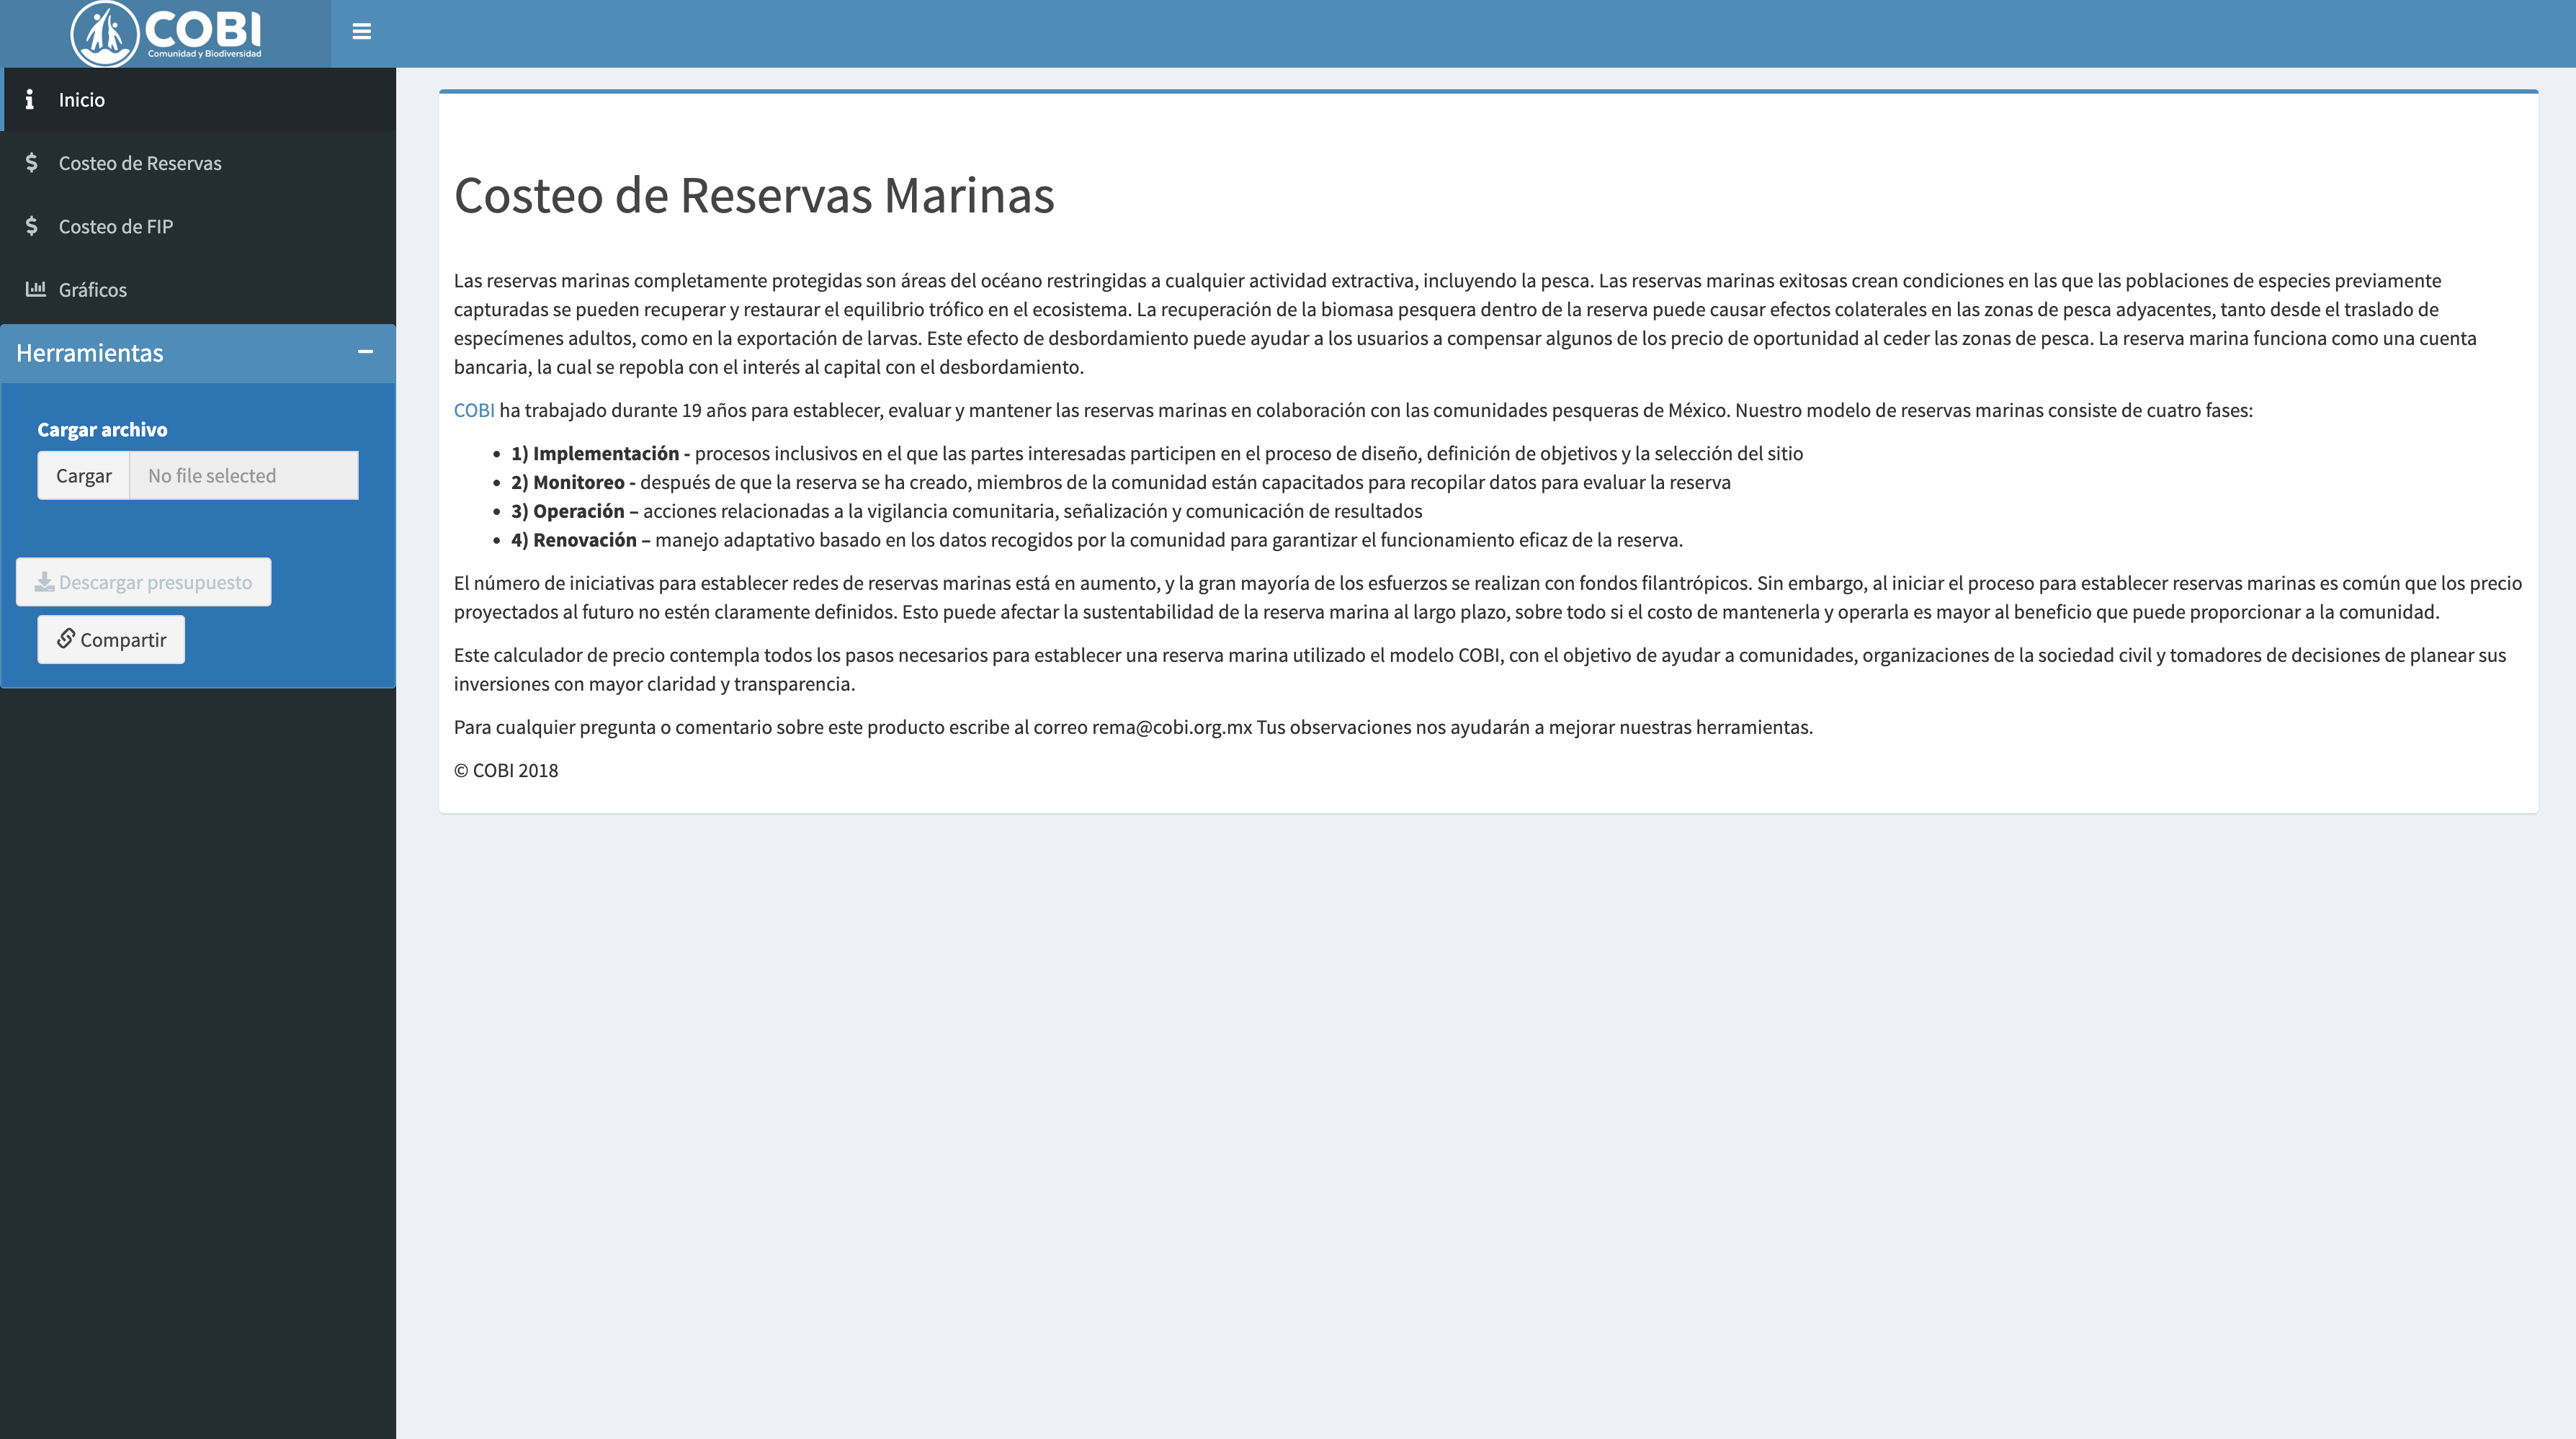
\includegraphics{images/Screen Shot 2022-07-25 at 2.43.50 PM.png}
\caption{\label{fig:landing-page}Página de bienvenida en la aplicación web.}
\end{figure}

\hypertarget{uxe1rea-de-trabajo}{%
\subsection{Área de trabajo}\label{uxe1rea-de-trabajo}}

Del lado derecho observarás el área de trabajo principal. Si estás trabajando en el llenado de un presupuesto, esta sección te mostrará los diferentes campos para que puedas ingresar los valores o explorar el presupuesto. Exploremos más a detalle cada una de estas.

La figura \ref{fig:filling-page} muestra el estado de la aplicación cuando el usuario ha seleccionado ``Costeo de Reservas'' en el menú lateral. En la zona superior del área de trabajo principal podrás observar tres pestañas con los nombres de ``Diseño'', ``Implementación'', y ``Seguimiento'', stas son las tres fases descritas en sección \ref{estructura}. La pestaña ``Duración'' está seleccionada, indicado por la barra azul sobre su nombre. En este punto, la aplicación te muestra una ventana titulada ``Duración de la fase'' en la que especificaremos la duración del a fase de diseño de las reservas marinas. La pestaña de diseño de FIPS es similar.

\begin{figure}
\centering
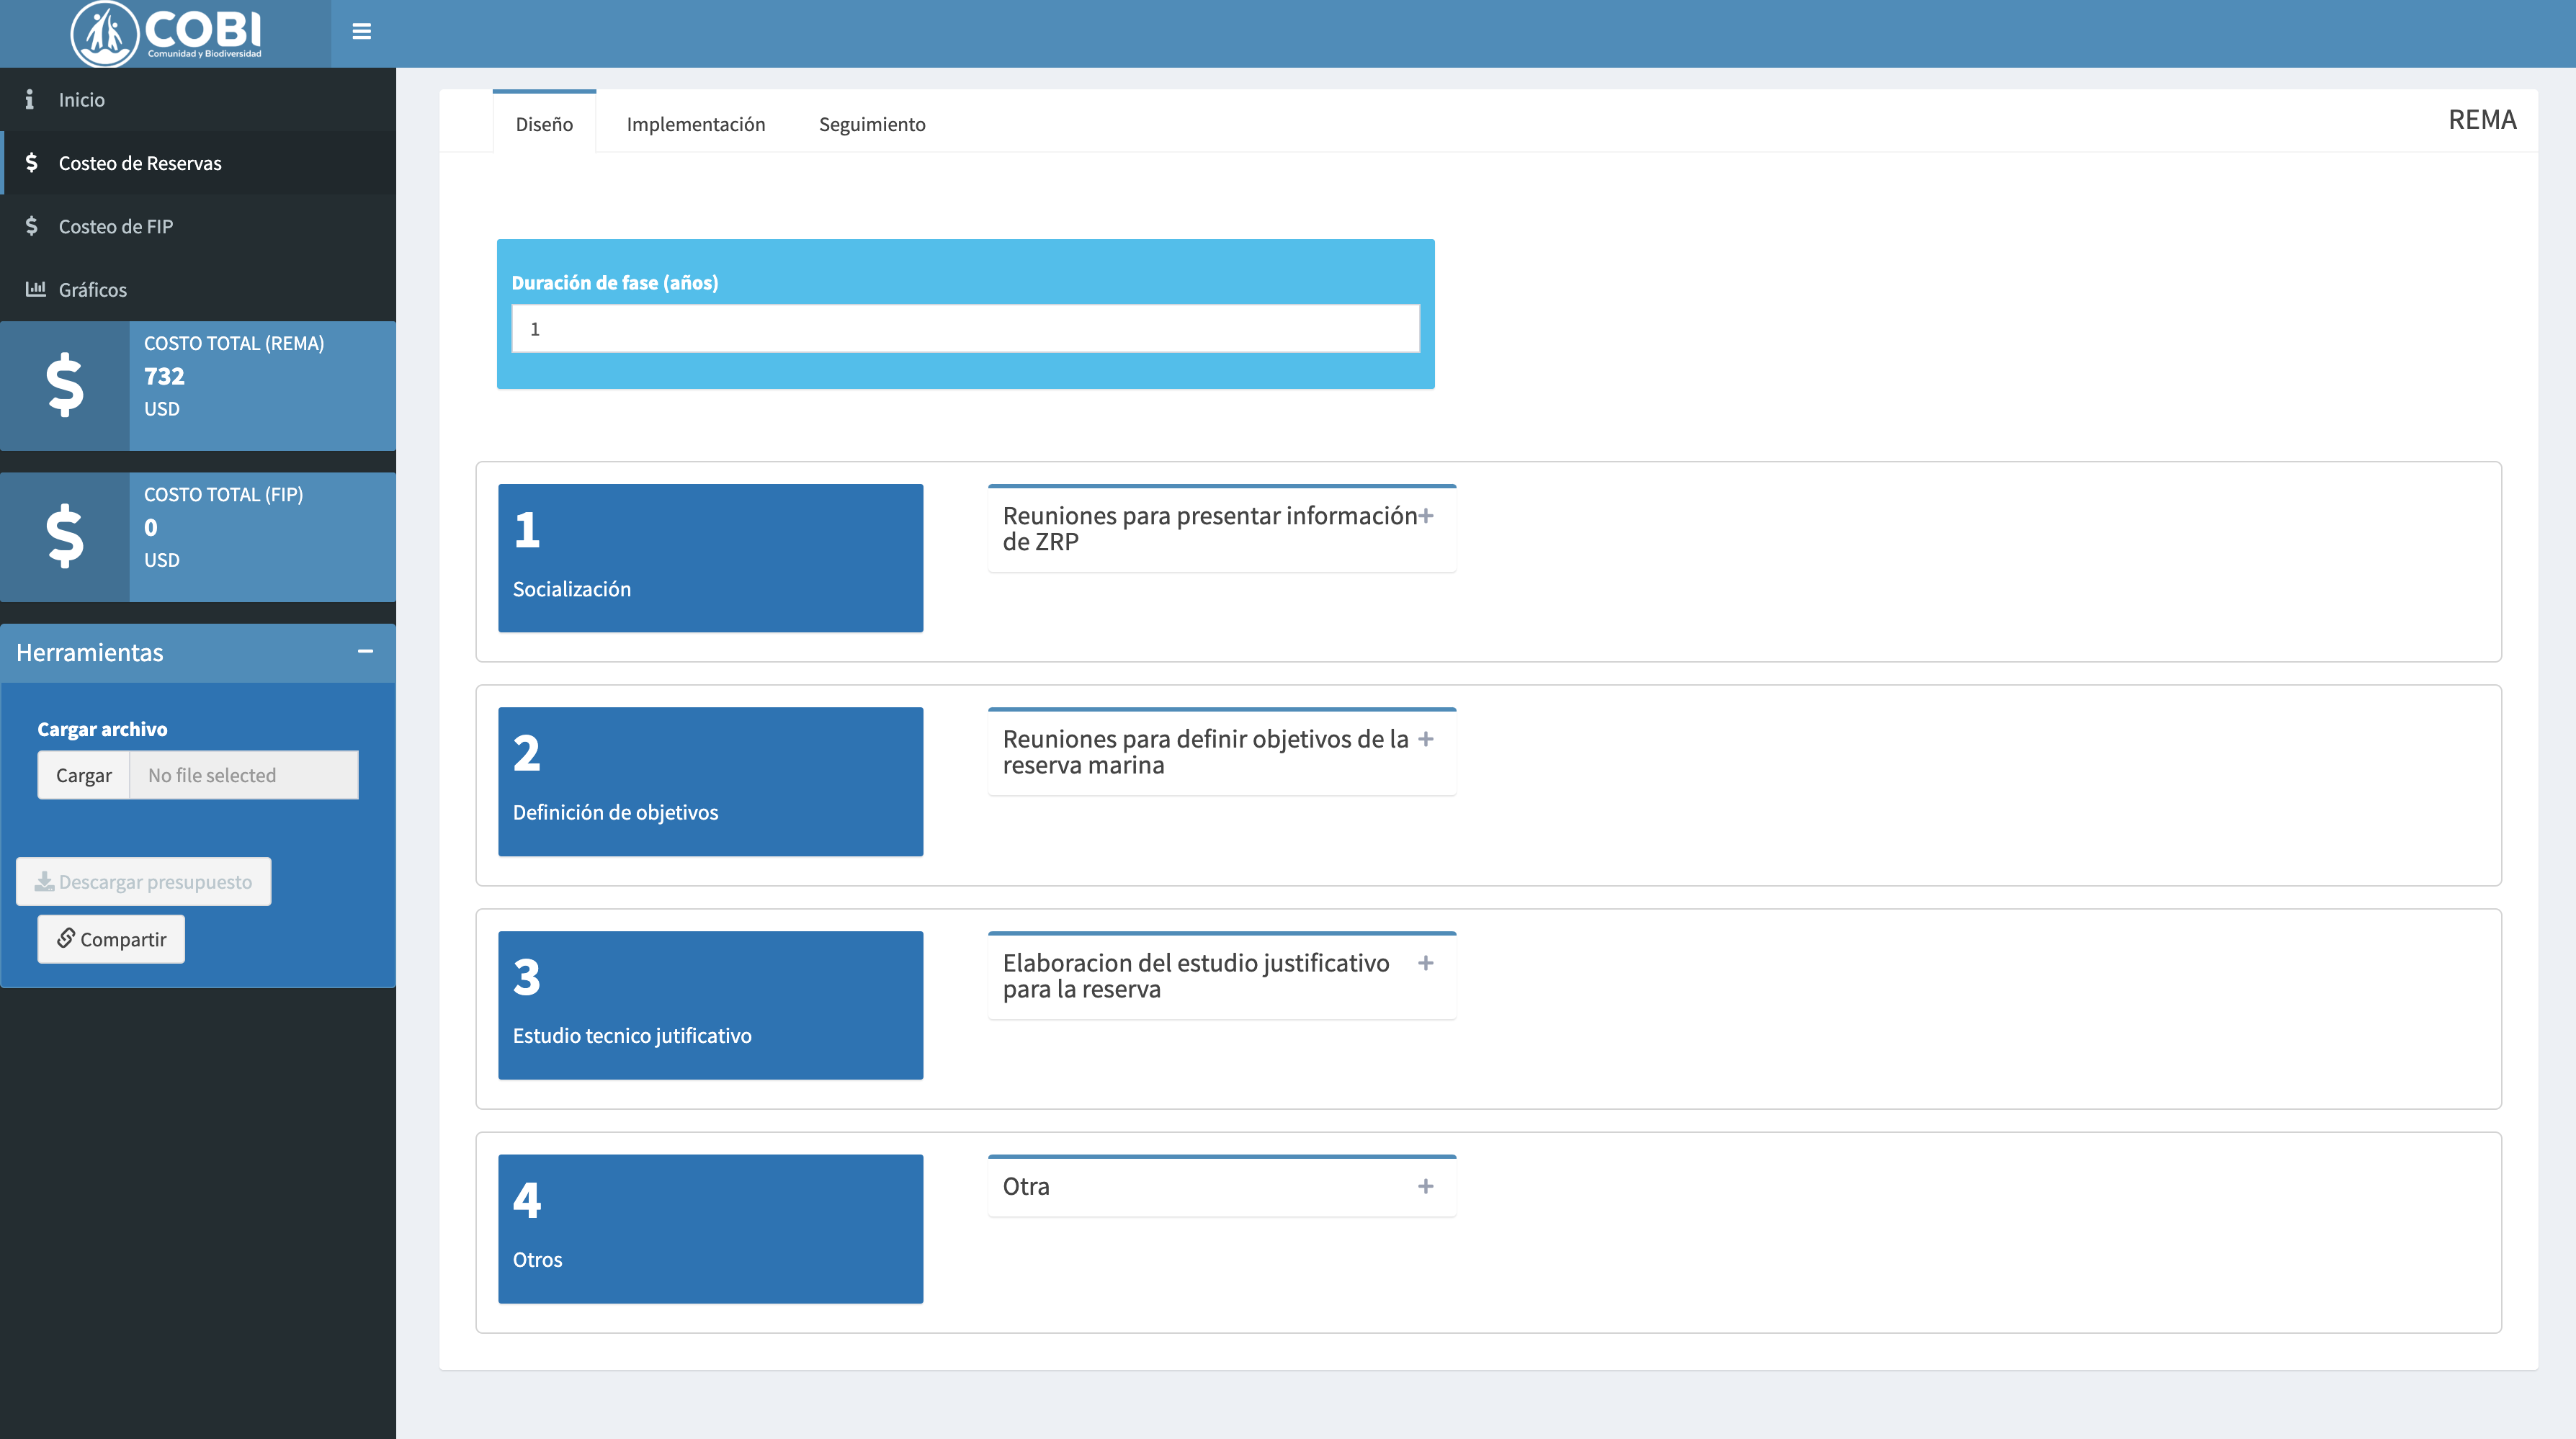
\includegraphics{images/Screen Shot 2022-07-25 at 2.56.05 PM.png}
\caption{\label{fig:filling-page}Página de llenado de datos en la aplicación web.}
\end{figure}

La fase de diseño de reservas marinas se subdivide en cuatro subfases, indicadas por los bloques azules del lado izquierdo. En este caso, el diseño de una reserva marina requiere de Socialización, Definicion de Objetivos, Elaboración de un Estudio Técnico Justificativo, y ``Otros'' (otros costos que el usuario puede incluir). Como dijimos en la sección \ref{estructura}, las subfases se dividen en actividades. Por ejemplo, la subfase de socialización cuenta con una única actividad: ``Reuniones para presentar información de ZRP''. Al hacer ``click'' en el signo de \textbf{+} a la derecha del título de la actividad, la aplicación despliega la lista de elementos a costear (Fig. \ref{fig:elements}), así como la frecuencia de la actividad.

\begin{figure}
\centering
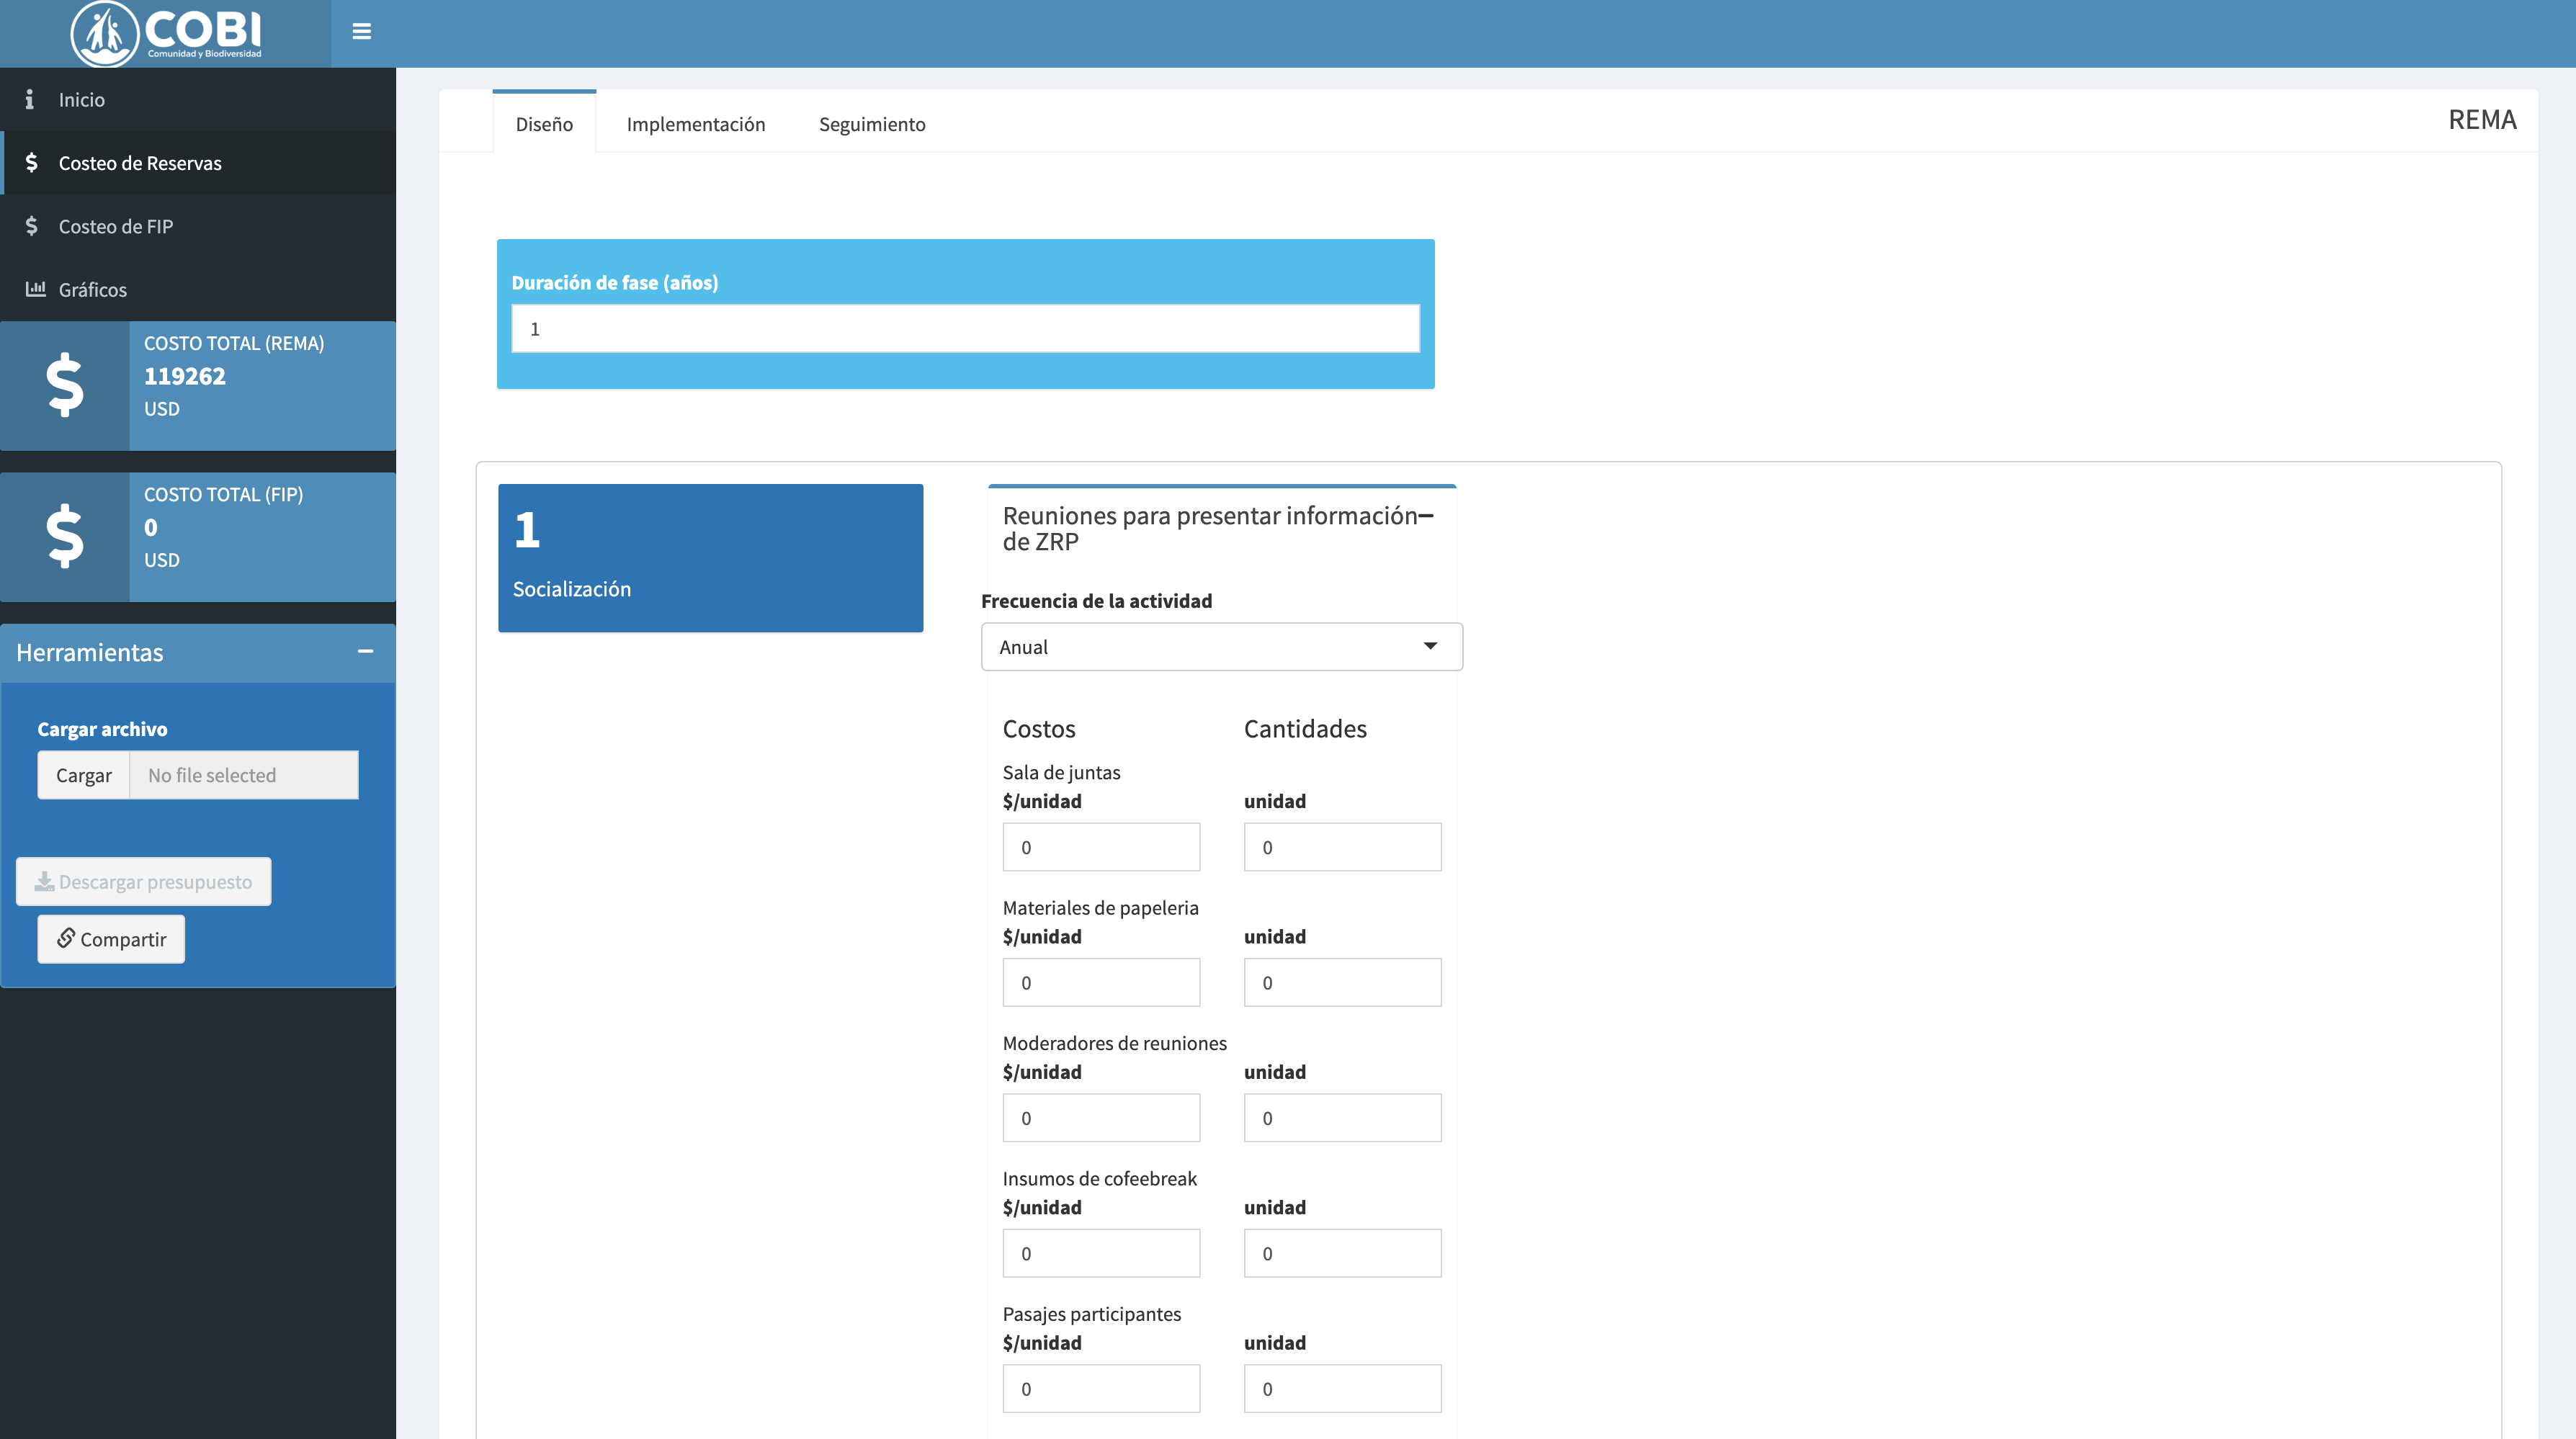
\includegraphics{images/Screen Shot 2022-07-25 at 3.08.10 PM.png}
\caption{\label{fig:elements}Elementos para la actividad de `Reuniones para presentar información de ZRP'.}
\end{figure}

La figura \ref{fig:viewing-page} muestra el último área de trabajo, donde podrás visualizar el presupuesto. Además, contiene una nueva característica de esta versión de la aplicación: Te permite dividir el presupuesto entre diferentes actores, y anticipar el monto de sus contribuciones.

\begin{figure}
\centering
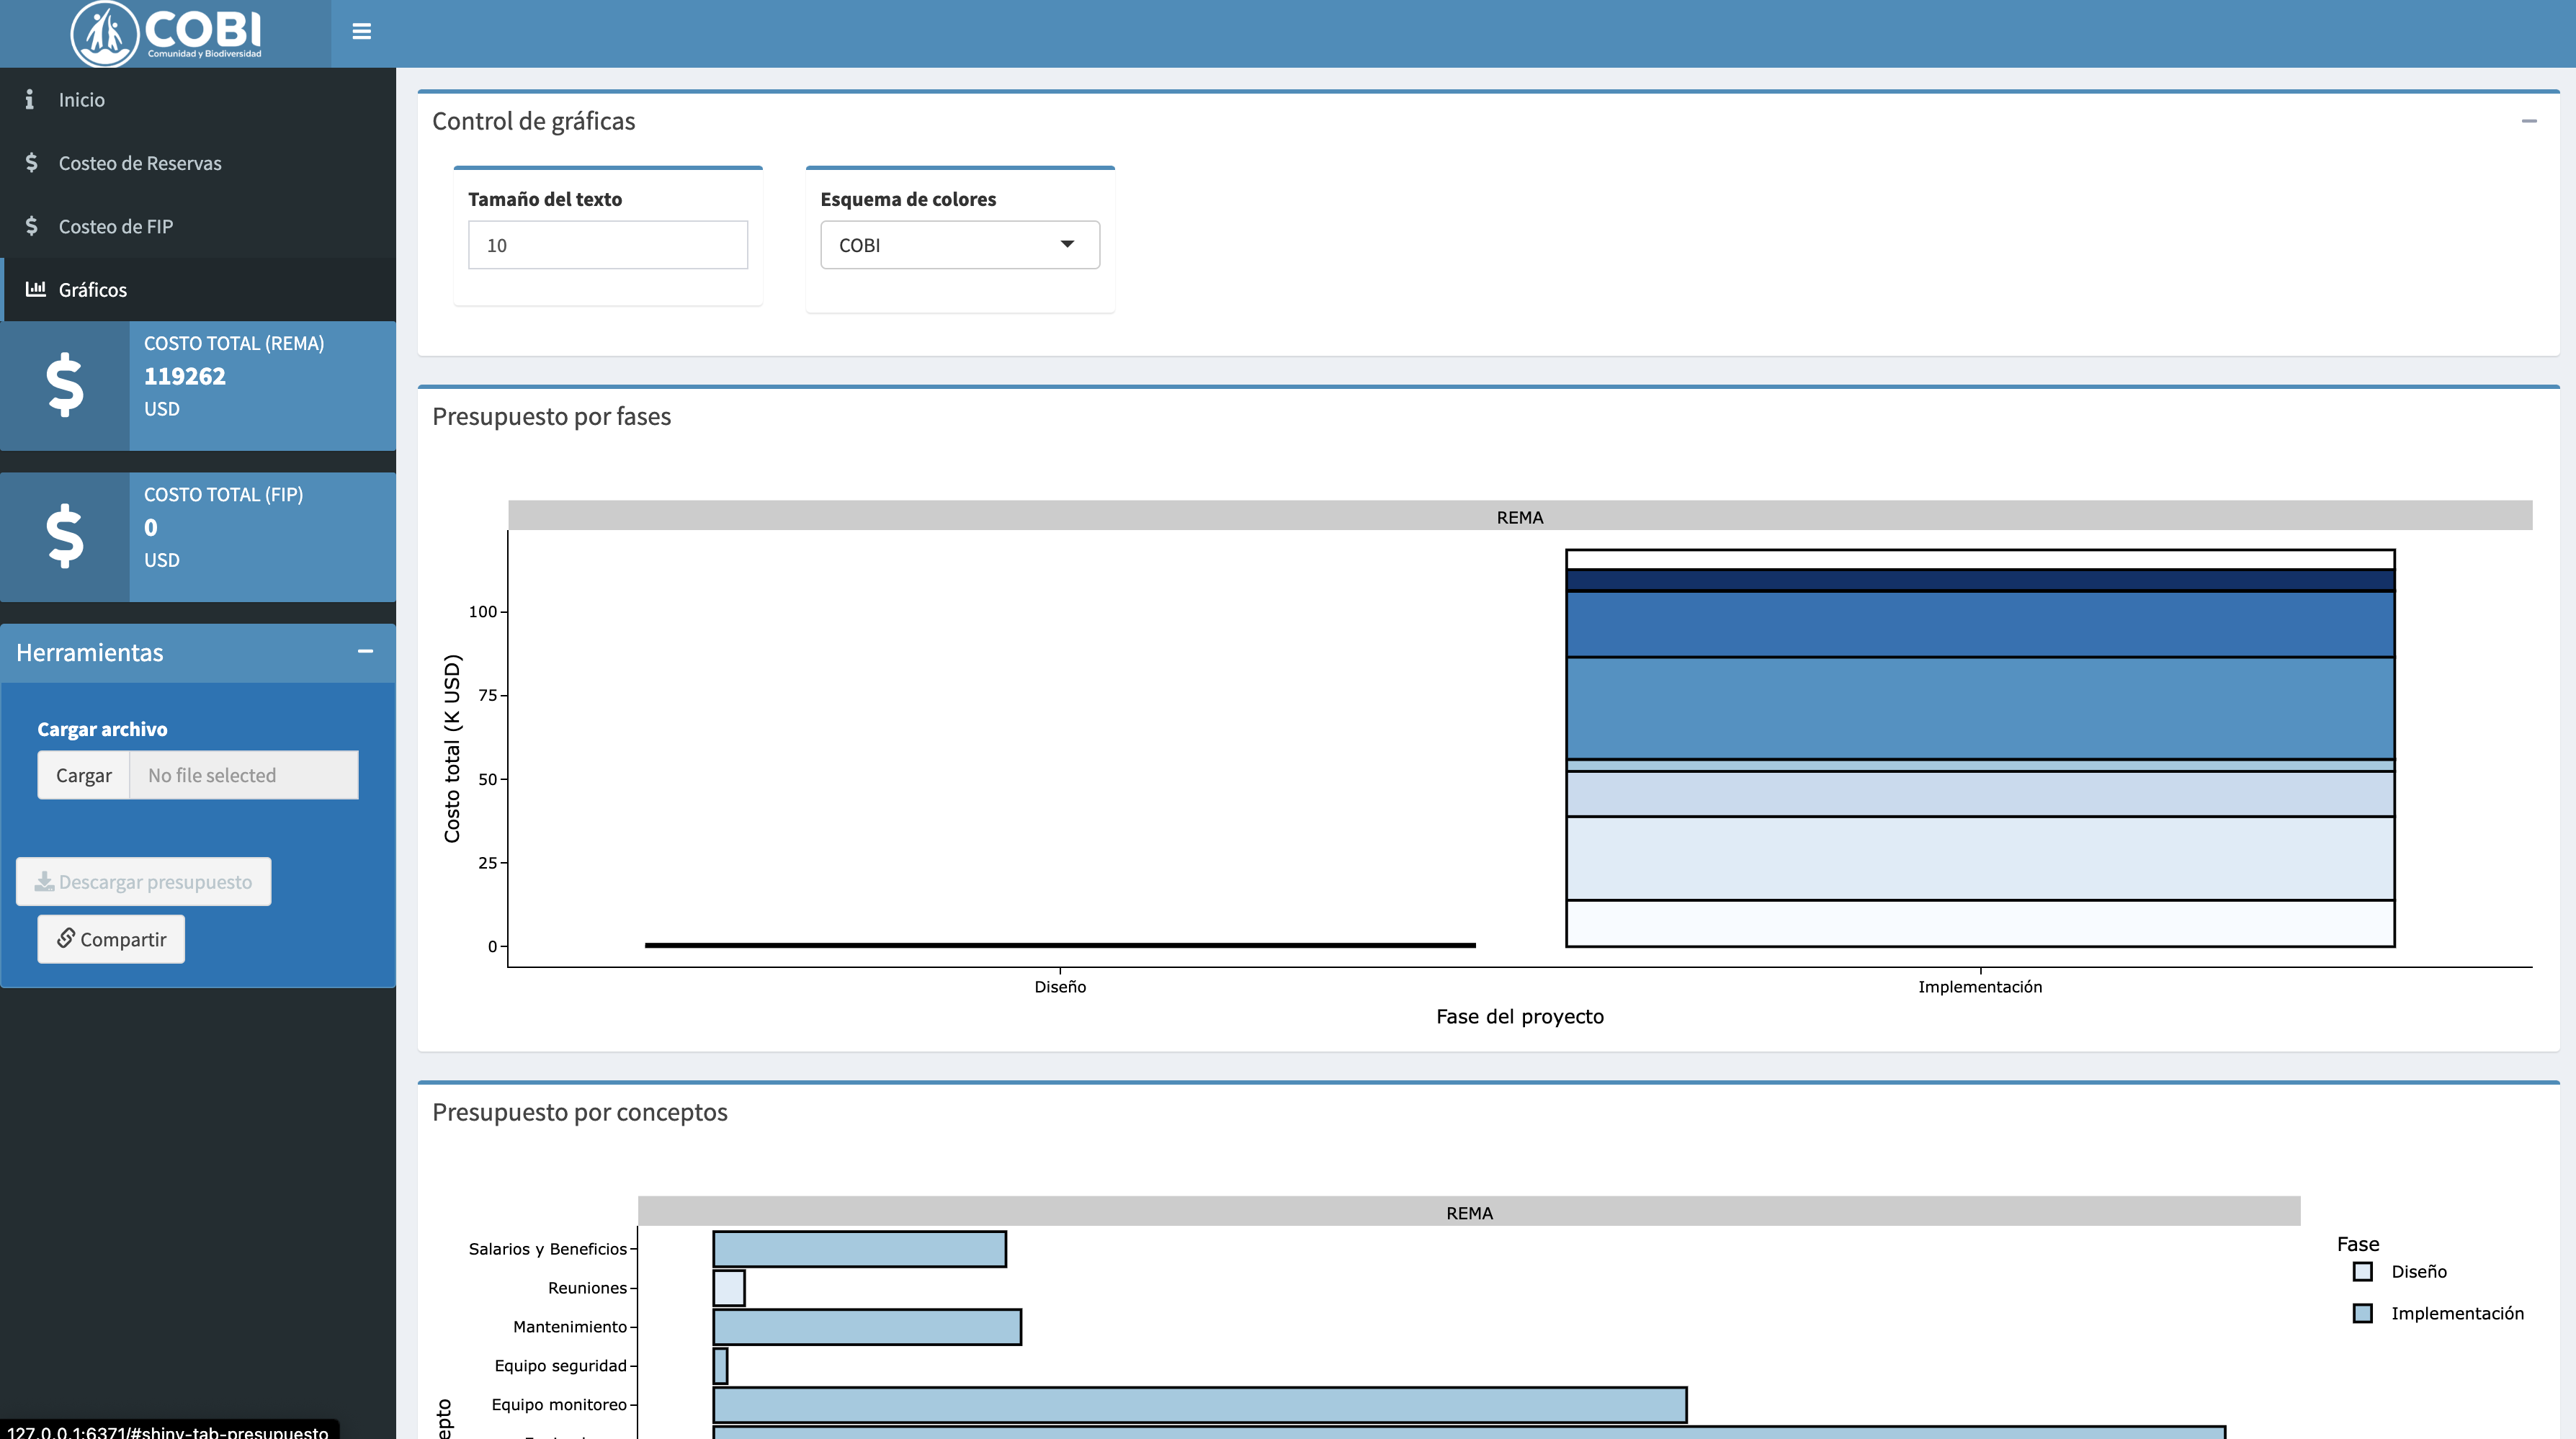
\includegraphics{images/Screen Shot 2022-07-25 at 2.56.18 PM.png}
\caption{\label{fig:viewing-page}Página de exploración de presupuesto en la aplicación web.}
\end{figure}

\hypertarget{llenado}{%
\chapter{Llenado de datos}\label{llenado}}

Llenado de datos

\begin{itemize}
\item
  Ejemplo REMA

  \begin{itemize}
  \item
    Solamente una fase
  \item
    Llenar un programa entero
  \end{itemize}
\item
  Ejemplo FIP

  \begin{itemize}
  \item
    Solamente una fase
  \item
    Módulo de intervenciones
  \end{itemize}
\end{itemize}

\hypertarget{explorar}{%
\chapter{Explorar el presupuesto}\label{explorar}}

Explorador de presupuesto

\begin{itemize}
\item
  Descripcion de grafica 1
\item
  Descripcion de grafica 2
\item
  Descripción del módulo de division presupuestal
\end{itemize}

\hypertarget{guardar}{%
\chapter{Guardar el progreso de un presupuesto}\label{guardar}}

Guardar el progreso de un evento presupuestal

\hypertarget{cargar}{%
\chapter{Cargar el estado de un presupuesto anterior}\label{cargar}}

Cargar un archivo anterior

\hypertarget{compartir}{%
\chapter{Compartir el estado de la aplicación}\label{compartir}}

Compartir el estado de la aplicación

  \bibliography{book.bib,packages.bib}

\end{document}
